\section{Ferramentas e tecnoloxías}

\begin{frame}{Linguaxe, librería e manexador de paquetes}
  \vfill
  \begin{itemize}
    \setlength{\itemsep}{1.6em}

    \item \destacado{Rust}: unha linguaxe de programación de sistemas. Compilado, fortemente tipado
    e con manexo automático de memoria sen \textit{garbage collector}.

    \item \destacado{Raylib}: librería para o desenvolvemento de videoxogos, coa que se manexa vídeo, audio e entrada de forma sinxela,
    puidendo compilarse para todo tipo de plataformas.

    \item \destacado{Nix}: manexador de paquetes declarativo,
    que permite definir contornas de desenvolvemento e imaxes completas dun sistema embebido de forma reproducibles.
  
  \end{itemize}
  \vfill
\end{frame}

\begin{frame}[plain,noframenumbering]{Anexo · Arquitectura de raylib}
  \begin{center}
    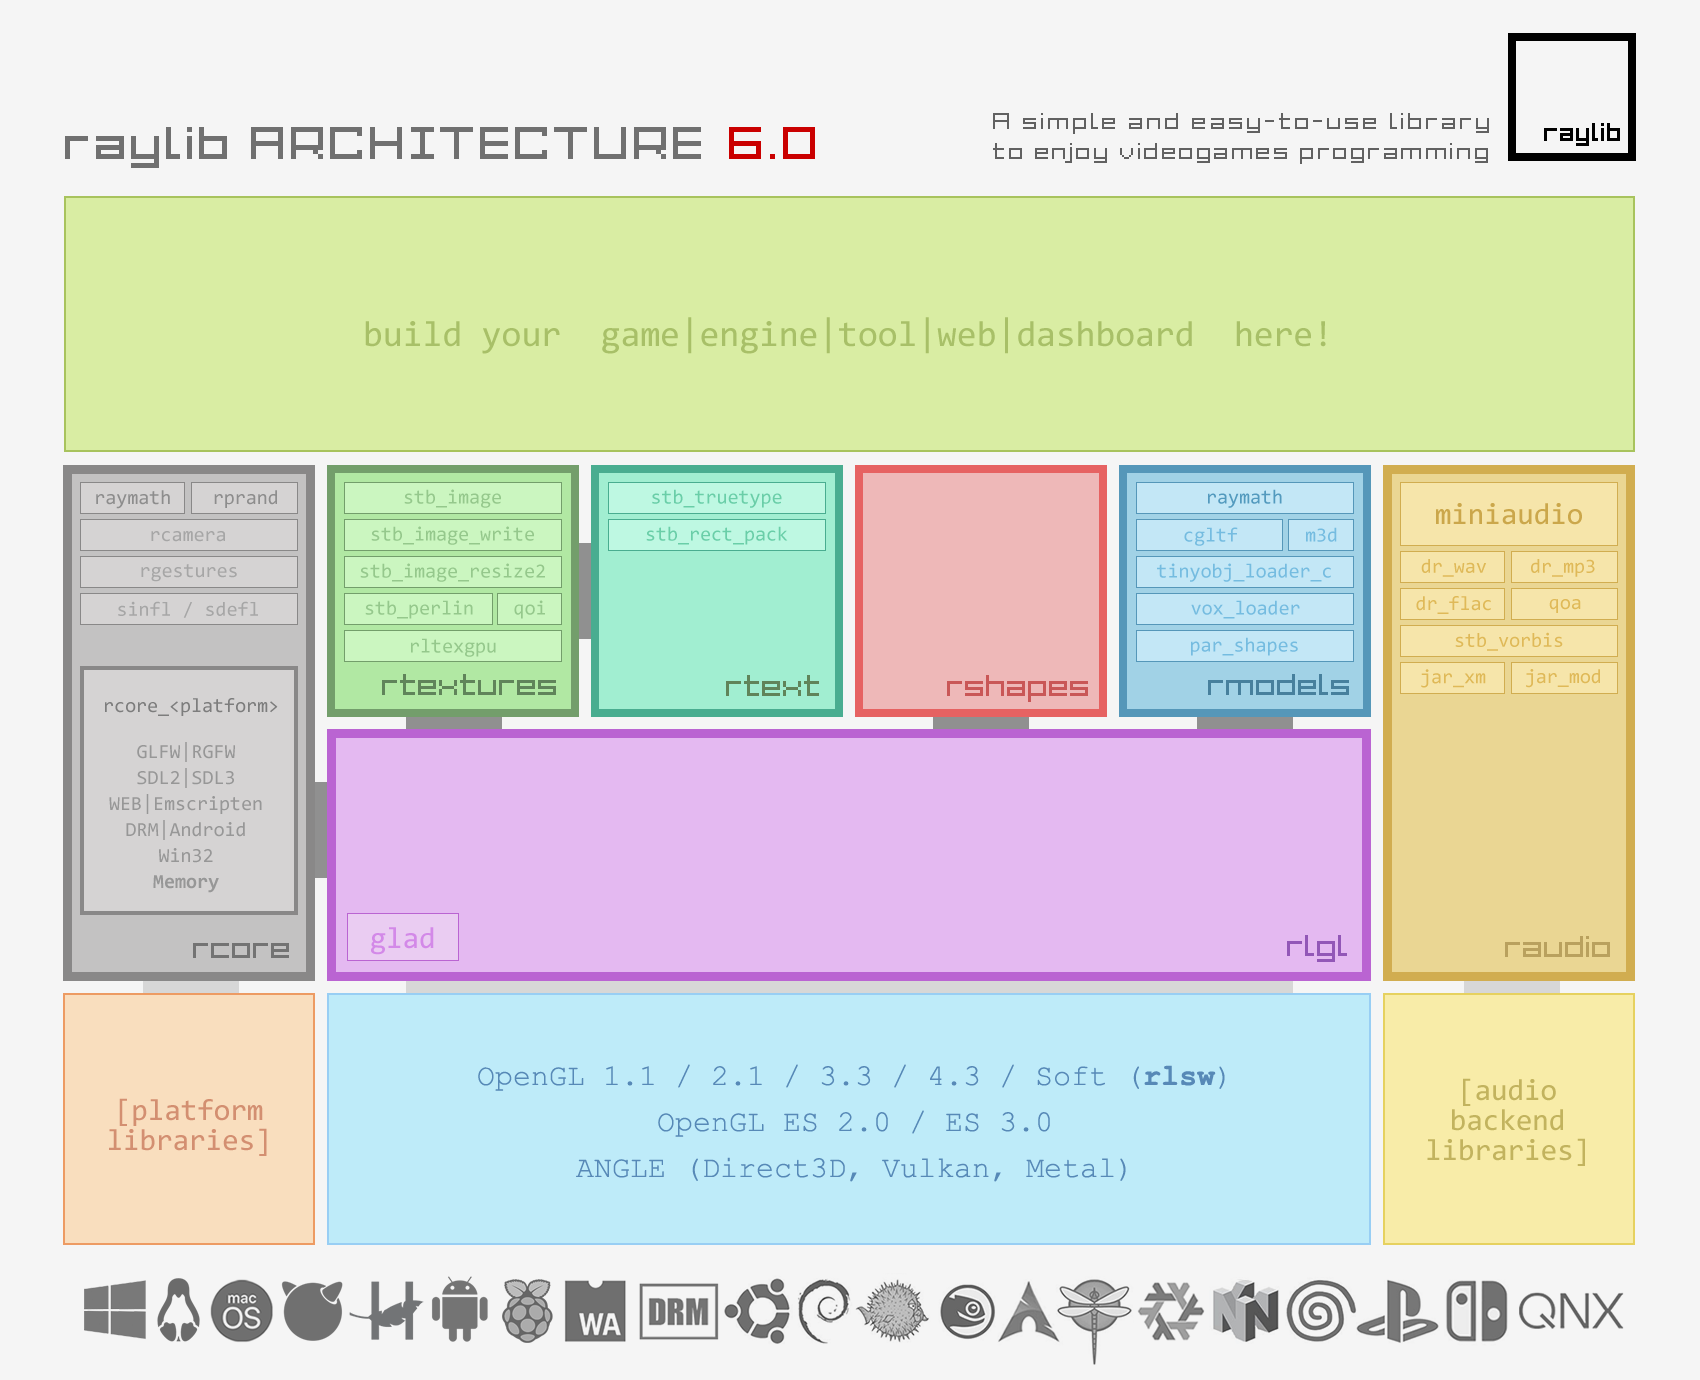
\includegraphics[height=0.78\textheight,keepaspectratio]{imaxes/raylib_architecture_v6.0.png}
  \end{center}
\end{frame}
